\chapter{Methods}

\section{ANNISA FATHORONI/1164067}
\subsection{Teori}
Penyelesaian Tugas Harian 5 ( No. 1-6 )
\begin{enumerate}
\item Random Forest Dan Ilustrasi Gambarnya
\begin{itemize}
\item Pengertian Random Forest:

Random forests atau random decision forests adalah metode pembelajaran ensembel untuk klasifikasi, regresi dan tugas-tugas lain yang beroperasi dengan membangun banyak pohon keputusan pada waktu pelatihan dan menghasilkan kelas yang merupakan mode kelas (klasifikasi) atau prediksi rata-rata (regresi) dari masing-masing pohon. Random decision forests tepat untuk kebiasaan pohon keputusan 'overfitting' pada set pelatihan mereka.

\item Ilustrasi Gambar Random Forest :

\begin{figure}[ht]
\centering
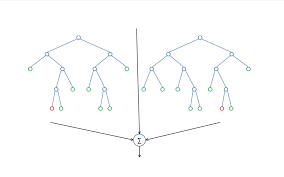
\includegraphics[scale=0.5]{figures/Chapter3AnnisaFathoroni1.png}
\caption{Random Forest}
\label{contoh}
\end{figure}

\end{itemize}

\item Cara Membaca Dataset

Berikut adalah cara membaca dataset :
\begin{itemize}
\item Buka Anaconda Navigator lalu jalankan Syder, kemudian import libraries yang dibutuhkan.
\item Masukkan kode python untuk membaca file csv, lalu jalankan

\begin{figure}[ht]
\centering
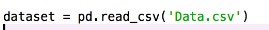
\includegraphics[scale=0.8]{figures/Chapter3AnnisaFathoroni5.jpeg}
\caption{Code Python}
\label{contoh}
\end{figure}

\item Maka pada window console akan menampilkan pesan berikut:

\begin{figure}[ht]
\centering
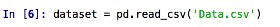
\includegraphics[scale=0.8]{figures/Chapter3AnnisaFathoroni6.jpeg}
\caption{Output}
\label{contoh}
\end{figure}

\item Dari explorer dapat terlihat dataset yang terimport.

\begin{figure}[ht]
\centering
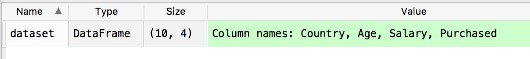
\includegraphics[scale=0.5]{figures/Chapter3AnnisaFathoroni7.jpeg}
\caption{Import Dataset}
\label{contoh}
\end{figure}

\item Lalu klik dataset cell, maka akan muncul seperti berikut :
\item Seperti yang terlihat pada gambar tersebut dataset ini memiliki Kolom Country, Age, dan Salary sebagai independent variable-nya dan kolom

\begin{figure}[ht]
\centering
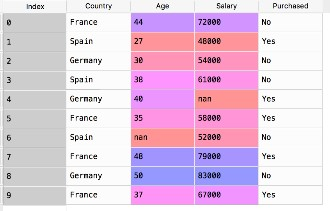
\includegraphics[scale=0.5]{figures/Chapter3AnnisaFathoroni8.jpeg}
\caption{Hasil Dataset Sel}
\label{contoh}
\end{figure}

\item Purchased sebagai dependent variable-nya.
\item Selanjutnya buat 2 matrix of features yang berisi values dari independent variable dan dependent variable.
\item Lalu tuliskan perintah berikut :

\begin{figure}[ht]
\centering
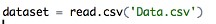
\includegraphics[scale=0.8]{figures/Chapter3AnnisaFathoroni9.jpeg}
\caption{Perintah}
\label{contoh}
\end{figure}

\item Perintah yang telah dibuat di atas akan membuat sebuah global environment baru dan muncul dataset.
\item Klik dataset tersebut maka muncul tabel berisi dataset.
\end{itemize}

\item Cross Validation

Cross-validation (CV) adalah metode statistik yang dapat digunakan untuk mengevaluasi kinerja model atau algoritma dimana data dipisahkan menjadi dua subset yaitu data proses pembelajaran dan data validasi / evaluasi. Model atau algoritma dilatih oleh subset pembelajaran dan divalidasi oleh subset validasi. Selanjutnya pemilihan jenis CV dapat didasarkan pada ukuran dataset. Biasanya CV K-fold digunakan karena dapat mengurangi waktu komputasi dengan tetap menjaga keakuratan estimasi.

\item Arti score 44\% pada random forest, 27\% pada decission tree dan 29\%dari SVM.

 Kalau maksud arti score 27\% pada decission tree adalah presentasi hasil dari perhitungan dataset, sedangkan maksud arti score 29\% dari SVM adalah hasil pendekatan jaringan saraf.  Hasil tersebut didapat dari hasil valdasi silang untuk memastikan bahwa membagi training test dengan cara yang berbeda. Sehingga didapat outputnya 44\% untuk hutan acak, 27\% untuk pohon keputusan, dan 29\% untuk SVM.

\item Confusion Matrix Dan Ilustrasinya
\begin{enumerate}
\item Perhitungan confusion matrix adalah sebagai berikut, akan saya beri contoh sederhana yaitu pengambilan keputusan untuk mendapatkan bantuan beasiswa. Saya menggunakan dua atribut, yaitu rekening listrik dan gaji. Ini adalah pohon keputusannya:
 
\begin{figure}[ht]
\centering
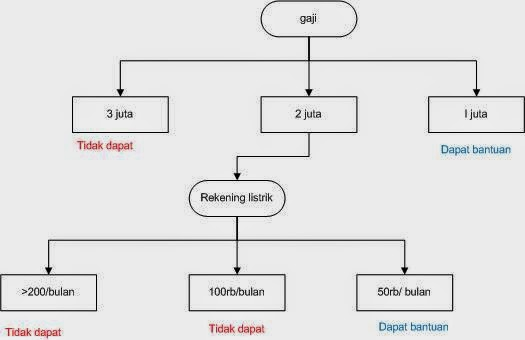
\includegraphics[scale=0.5]{figures/Chapter3AnnisaFathoroni2.jpg}
\caption{Pohon Keputusan}
\label{contoh}
\end{figure}
\end{enumerate}

Kemudian data testingnya adalah

\begin{figure}[ht]
\centering
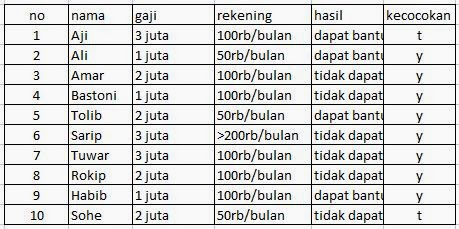
\includegraphics[scale=0.5]{figures/Chapter3AnnisaFathoroni3.jpg}
\caption{Data Testing}
\label{contoh}
\end{figure}

Yang pertama kita lakukan yaitu mencari 4 nilai yaitu a,b,c, dan d:

a= 5

b= 1

c= 1

d= 3

Kemudian kita dapat mencari nilai Recall, Precision, accuracy dan Error Rate

Recall =3/(1+3) = 0,75

Precision = 3/(1+3) = 0,75

Accuracy =(5+3)/(5+1+1+3) = 0,8

Error Rate =(1+1)/(5+1+1+3) = 0,2

\item Voting Random Forest Dan Ilustrasi Gambarnya.

\begin{itemize}
\item Pengertian Voting pada Random Forest

Metode ensemble dapat mencapai akurasi tinggi dengan membangun beberapa pengklasifikasi dan menjalankan masing-masing secara mandiri. Ketika classifier membuat keputusan, Anda dapat memanfaatkan yang terbaik keputusan umum dan rata-rata. Jika kita menggunakan metode yang paling umum, itu disebut voting

\item Ilustrasi Gambar Voting Random Forest :
\begin{figure}[ht]
\centering
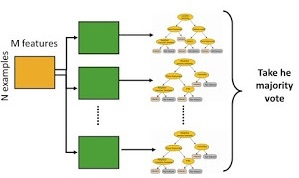
\includegraphics[scale=0.8]{figures/Chapter3AnnisaFathoroni4.jpg}
\caption{Voting Random Forest}
\label{contoh}
\end{figure}
\end{itemize}
\end{enumerate}

\section{Tasya Wiendhyra/1164086}
HARI PERTAMA TEORI
\section{Random Forest Dan Contohnya}
\subsection{Pengertian}
Random Forest adalah konstruk data yang diterapkan pada machine learning yang mengembangkan sejumlah besar pohon keputusan acak yang menganalisis sekumpulan variabel. Jenis algoritma ini membantu meningkatkan cara teknologi menganalisis data yang kompleks. Juga merupakan algoritma machine learning yang fleksibel, mudah digunakan, bahkan tanpa penyetelan hyper-parameter, dengan hasil yang baik. Ini juga merupakan salah satu algoritma yang paling banyak digunakan, karena kesederhanaan dan faktanya dapat digunakan untuk tugas klasifikasi dan regresi.\\
Dibawah ini merupakan salah satu ilustrasi penggunaan Random Forest yang saya lakukan untuk memprediksi apakah uang kertas bank otentik atau tidak berdasarkan pada empat atribut.
Ini merupakan hasil dari ilustrasi Random Forest pada Spyder
\begin{figure}[ht]
\centering
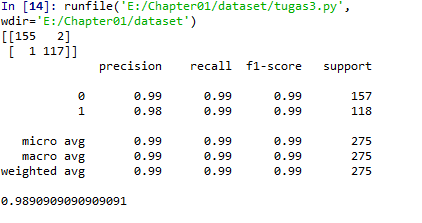
\includegraphics[scale=0.5]{figures/teori1.png}
\caption{Random Forest Spyder}
\label{Contoh}
\end{figure}
\par
Setelah di plotting hasilnya seperti berikut
\begin{figure}[ht]
\centering
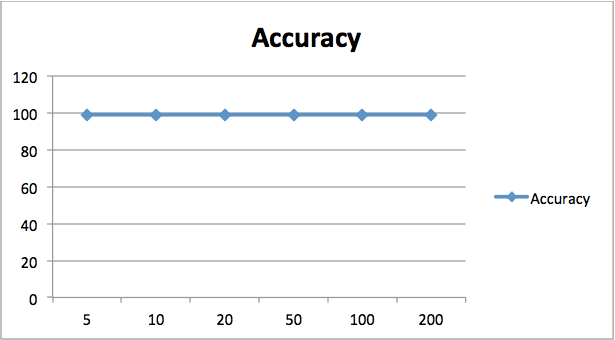
\includegraphics[scale=0.5]{figures/teori2.png}
\caption{Random Forest Graphic}
\label{Contoh}
\end{figure}

\section{Dataset}
\subsection{Pengertian Dataset}
Dataset adalah kumpulan data. Paling umum satu data set sesuai dengan isi tabel database tunggal, atau matriks data statistik tunggal, di mana setiap kolom tabel mewakili variabel tertentu, dan setiap baris sesuai dengan anggota tertentu dari dataset yang dipertanyakan.
\subsection{Cara Membaca Dataset Dan Arti Setiap File Dan Isi Field Masing Masing File}
\begin{enumerate}
\item
Gunakan librari Pandas pada python untuk dapat membaca dataset dengan format text file.
\item
Setelah itu, buat variabel baru "dataset" yang berisikan perintah untuk membaca file csv. seperti berikut
\begin{figure}[ht]
\centering
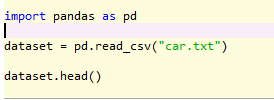
\includegraphics[scale=0.5]{figures/teori3.png}
\caption{Dataset Pandas}
\label{Contoh}
\end{figure}
\par
Pada gambar diatas dapat dijelaskan bahwa :\\
\begin{itemize}
\item
Memanggil Librari Panda untuk membaca dataset
\item
Membuat variabel "Dataset" yang berisikan pdreadcsv untuk membaca dataset. Pada contoh ini menggunakan txt tapi tetap bisa membaca datasetnya, mengapa? Karena pada saat dijalankan librari panda secara otomatis akan mengubah data dalam bentuk text file ke format csv.
\end{itemize}
\item
Setelah di run akan muncul hasil seperti berikut :
\begin{figure}[ht]
\centering
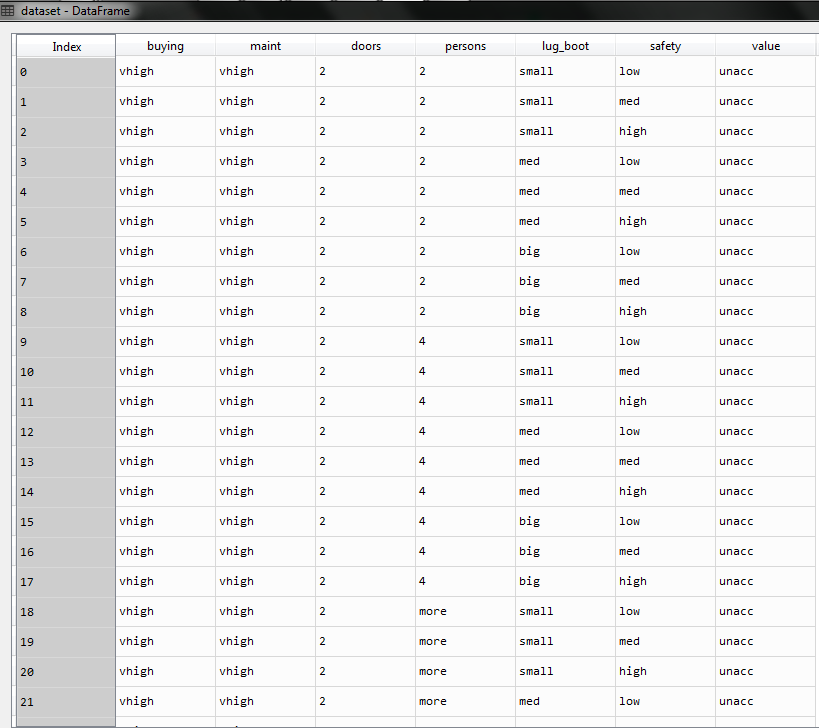
\includegraphics[scale=0.5]{figures/teori4.png}
\caption{Dataset Pandas}
\label{Contoh}
\end{figure}
\par
Pertama tama gambar diatas merupakan dataset yang digunakan untuk evaluasi mobil setelah dibuat untuk mengecek dan menguji induksi konstruktif dan metode penemuan struktur. Datasetnya dapat didapatkan dari laman https://archive.ics.uci.edu/ml/datasets/Car+Evaluation.\\
Penjelasan dari isi field diatas adalah sebagai berikut :\\
\begin{itemize}
\item
Atribut Index merupakan atribut otomatis untuk penomoran data yang ada.
\item
Atribut Buying merupakan harga beli dari mobil tersebut. dengan value : v high/Sangat mahal,high/mahal,med/Cukup, low/Murah.
\item
Atribut Maint merupakan harga perawatan dari mobil tersebut, dengan value sama seperti pada atribut Buying.
\item
Atribut Doors merupakan jumlah pintu yang terdapat pada mobil, dengan value 2,3,4,5 more atau lebih dari 5.
\item
Atribut Persons merupakan kapasitas orang yang bisa masuk kedapalm mobil, dengan value 2,4, more /lebih.
\item
Atribut Lug Boot merupakan ukuran bagasi boot mobil, dengan value small,med,big.
\item
Atribut Safety merupakan perkiraan keselamatan mobil, dengan value low,med,high.
\item
Yang terakhir yaitu Value, yang dimana merupakan merupakan Class nya atau disebut dengan targetnya menyatakan apakah mobil tersebut dapat diterima atau tidak dan apakah mobil tersebut bagus atau tidak, dengan value unacc, acc, good,v good .
\end{itemize}
\end{enumerate}

\section{Cross Validation}
Cross Validation adalah prosedur resampling yang digunakan untuk mengevaluasi model machine learning pada sampel data yang terbatas. Prosedur ini memiliki parameter tunggal yang disebut k yang mengacu pada jumlah grup tempat sampel data yang akan dibagi. Karena itu, prosedur ini sering disebut k-fold cross-validation.\\
Proses penentuan apakah hasil numerik yang mengukur hubungan yang dihipotesiskan antar variabel, dapat diterima sebagai deskripsi data, dikenal sebagai Validationi. Umumnya, estimasi kesalahan untuk model dibuat setelah training, lebih dikenal sebagai evaluasi residu. Dalam proses ini, estimasi numerik dari perbedaan respons yang diprediksi dan yang asli dilakukan, juga disebut kesalahan training. Namun, ini hanya memberi kita gambaran tentang seberapa baik model kita pada data yang digunakan untuk melatihnya. Sekarang mungkin bahwa model tersebut kurang cocok atau overfitting data. Jadi, masalah dengan teknik evaluasi ini adalah bahwa itu tidak memberikan indikasi seberapa baik pelajar akan menggeneralisasi ke set data independen / tidak terlihat. Model ini dikenal sebagai Cross Validation.

\section{Arti Score 44\% Pada Random Forest, 27\% Pada Decission Tree Dan 29\% Dari SVM}
Itu merupakan presentase keakurasian prediksi yang dilakukan pada saat testing menggunakan label pada dataset yang digunakan. Score merupakan mendefinisikan aturan evaluasi model. Maka pada saat dijalankan akan muncuk persentase tersebut yang menunjukan keakurasian atau keberhasilan dari prediksi yang dilakukan. Jika menggunakan Random Forest maka hasilnya 40\% , jika menggunakan Decission Tree hasil prediksinya yaitu 27\% dan pada SVM 29\% .

\section{Confusion Matriks}
\subsection{Confusion Matriks Dan Contohnya}
Perthitungan Confusion Matriks dapat dilakukan sebagai berikut. Disini saya menggunakan data yang dibuat sendiri untuk menampilkan data aktual dan prediksi.
\begin{itemize}
\item
Import librari Pandas, Matplotlib, dan Numpy.
\item
Buat variabel y actu yang berisikan data aktual.
\item
Buat variabel y pred berisikan data yang akan dijadikan sebagai prediksi.
\item
Buat variabel df confusion yang berisikan crosstab untuk membangun tabel tabulasi silang yang dapat menunjukkan frekuensi kemunculan kelompok data tertentu.
\item
Pada variabel df confusion definisikan lagi nama baris yaitu Actual dan kolomnya Predicted
\item
Kemudian definisikan suatu fungsi yang diberi nama plot confusion matrix yang berisikan pendefinisian confusion matrix dan juga akan di plotting. untuk code lengkapnya sebagai berikut 
\begin{verbatim}
import numpy as np
import matplotlib.pyplot as plt
import pandas as pd

y_actu = pd.Series([2, 0, 2, 2, 0, 1, 1, 2, 2, 0, 1, 2], name='Actual')
y_pred = pd.Series([0, 0, 2, 1, 0, 2, 1, 0, 2, 0, 2, 2], name='Predicted')
df_confusion = pd.crosstab(y_actu, y_pred)

df_confusion = pd.crosstab(y_actu, y_pred, rownames=['Actual'], colnames=['Predicted'], margins=True)

def plot_confusion_matrix(df_confusion, title='Confusion matrix', cmap=plt.cm.gray_r):
    plt.matshow(df_confusion, cmap=cmap) # imshow
    #plt.title(title)
    plt.colorbar()
    tick_marks = np.arange(len(df_confusion.columns))
    plt.xticks(tick_marks, df_confusion.columns, rotation=45)
    plt.yticks(tick_marks, df_confusion.index)
    #plt.tight_layout()
    plt.ylabel(df_confusion.index.name)
    plt.xlabel(df_confusion.columns.name)

plot_confusion_matrix(df_confusion)

plt.show()
\end{verbatim}

\par

Hasilnya akan seperti berikut :
\begin{figure}[ht]
\centering
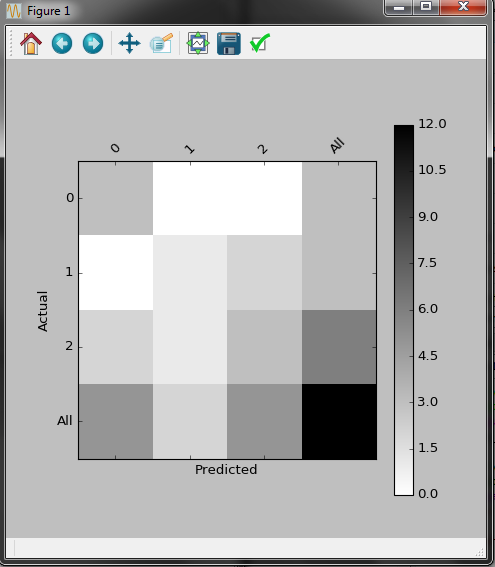
\includegraphics[scale=0.5]{figures/teori5.png}
\caption{Confusion Matrix}
\label{Contoh}
\end{figure}
\end{itemize}

\section{Voting Pada Random Forest}
\subsection{Pengertian}
Voting yaitu suara untuk setiap target yang diprediksi pada saat melakukan Random Forest. Pertimbangkan target prediksi dengan voting tertinggi sebagai prediksi akhir dari algoritma random forest.
\subsection{Contoh}
\begin{itemize}
\item
Untuk menggunakan Voting pada Random Forest dapat dilihat code berikut. Disini saya mengilustrasikan voting untuk berbagai macam algoritma terutama Random Forest.
\begin{verbatim}
import numpy as np
import matplotlib.pyplot as plt

from sklearn.linear_model import LogisticRegression
from sklearn.naive_bayes import GaussianNB
from sklearn.ensemble import RandomForestClassifier
from sklearn.ensemble import VotingClassifier

clf1 = LogisticRegression(solver='lbfgs', max_iter=1000, random_state=123)
clf2 = RandomForestClassifier(n_estimators=100, random_state=123)
clf3 = GaussianNB()
X = np.array([[-1.0, -1.0], [-1.2, -1.4], [-3.4, -2.2], [1.1, 1.2]])
y = np.array([1, 1, 2, 2])

eclf = VotingClassifier(estimators=[('lr', clf1), ('rf', clf2), ('gnb', clf3)],
                        voting='soft',
                        weights=[1, 1, 5])

# predict class probabilities for all classifiers
probas = [c.fit(X, y).predict_proba(X) for c in (clf1, clf2, clf3, eclf)]

# get class probabilities for the first sample in the dataset
class1_1 = [pr[0, 0] for pr in probas]
class2_1 = [pr[0, 1] for pr in probas]


# plotting

N = 4  # number of groups
ind = np.arange(N)  # group positions
width = 0.35  # bar width

fig, ax = plt.subplots()

# bars for classifier 1-3
p1 = ax.bar(ind, np.hstack(([class1_1[:-1], [0]])), width,
            color='green', edgecolor='k')
p2 = ax.bar(ind + width, np.hstack(([class2_1[:-1], [0]])), width,
            color='lightgreen', edgecolor='k')

# bars for VotingClassifier
p3 = ax.bar(ind, [0, 0, 0, class1_1[-1]], width,
            color='blue', edgecolor='k')
p4 = ax.bar(ind + width, [0, 0, 0, class2_1[-1]], width,
            color='steelblue', edgecolor='k')

# plot annotations
plt.axvline(2.8, color='k', linestyle='dashed')
ax.set_xticks(ind + width)
ax.set_xticklabels(['LogisticRegression\nweight 1',
                    'GaussianNB\nweight 1',
                    'RandomForestClassifier\nweight 5',
                    'VotingClassifier\n(average probabilities)'],
                   rotation=40,
                   ha='right')
plt.ylim([0, 1])
plt.title('Class probabilities for sample 1 by different classifiers')
plt.legend([p1[0], p2[0]], ['class 1', 'class 2'], loc='upper left')
plt.tight_layout()
plt.show()
\end{verbatim}
\item
Hasilnya sebagai berikut 
\begin{figure}[ht]
\centering
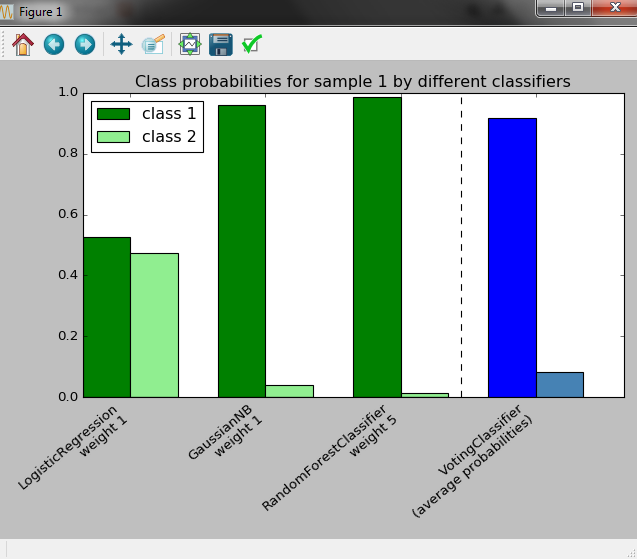
\includegraphics[scale=0.5]{figures/teori6.png}
\caption{Voting Random Forest}
\label{Contoh}
\end{figure}
\end{itemize}





